
%% bare_conf_compsoc.tex
%% V1.4b
%% 2015/08/26
%% by Michael Shell
%% See:
%% http://www.michaelshell.org/
%% for current contact information.
%%
%% This is a skeleton file demonstrating the use of IEEEtran.cls
%% (requires IEEEtran.cls version 1.8b or later) with an IEEE Computer
%% Society conference paper.
%%
%% Support sites:
%% http://www.michaelshell.org/tex/ieeetran/
%% http://www.ctan.org/pkg/ieeetran
%% and
%% http://www.ieee.org/

%%*************************************************************************
%% Legal Notice:
%% This code is offered as-is without any warranty either expressed or
%% implied; without even the implied warranty of MERCHANTABILITY or
%% FITNESS FOR A PARTICULAR PURPOSE!
%% User assumes all risk.
%% In no event shall the IEEE or any contributor to this code be liable for
%% any damages or losses, including, but not limited to, incidental,
%% consequential, or any other damages, resulting from the use or misuse
%% of any information contained here.
%%
%% All comments are the opinions of their respective authors and are not
%% necessarily endorsed by the IEEE.
%%
%% This work is distributed under the LaTeX Project Public License (LPPL)
%% ( http://www.latex-project.org/ ) version 1.3, and may be freely used,
%% distributed and modified. A copy of the LPPL, version 1.3, is included
%% in the base LaTeX documentation of all distributions of LaTeX released
%% 2003/12/01 or later.
%% Retain all contribution notices and credits.
%% ** Modified files should be clearly indicated as such, including  **
%% ** renaming them and changing author support contact information. **
%%*************************************************************************


% *** Authors should verify (and, if needed, correct) their LaTeX system  ***
% *** with the testflow diagnostic prior to trusting their LaTeX platform ***
% *** with production work. The IEEE's font choices and paper sizes can   ***
% *** trigger bugs that do not appear when using other class files.       ***                          ***
% The testflow support page is at:
% http://www.michaelshell.org/tex/testflow/



\documentclass[conference,compsoc]{IEEEtran}
% Some/most Computer Society conferences require the compsoc mode option,
% but others may want the standard conference format.
%
% If IEEEtran.cls has not been installed into the LaTeX system files,
% manually specify the path to it like:
% \documentclass[conference,compsoc]{../sty/IEEEtran}





% Some very useful LaTeX packages include:
% (uncomment the ones you want to load)


% *** MISC UTILITY PACKAGES ***
%
%\usepackage{ifpdf}
% Heiko Oberdiek's ifpdf.sty is very useful if you need conditional
% compilation based on whether the output is pdf or dvi.
% usage:
% \ifpdf
%   % pdf code
% \else
%   % dvi code
% \fi
% The latest version of ifpdf.sty can be obtained from:
% http://www.ctan.org/pkg/ifpdf
% Also, note that IEEEtran.cls V1.7 and later provides a builtin
% \ifCLASSINFOpdf conditional that works the same way.
% When switching from latex to pdflatex and vice-versa, the compiler may
% have to be run twice to clear warning/error messages.






% *** CITATION PACKAGES ***
%
\ifCLASSOPTIONcompsoc
  % IEEE Computer Society needs nocompress option
  % requires cite.sty v4.0 or later (November 2003)
  \usepackage[nocompress]{cite}
\else
  % normal IEEE
  \usepackage{cite}
\fi

\usepackage{verbatim}
\usepackage{amsmath}
\usepackage{amssymb}
\usepackage{graphicx}
\usepackage{array}
% cite.sty was written by Donald Arseneau
% V1.6 and later of IEEEtran pre-defines the format of the cite.sty package
% \cite{} output to follow that of the IEEE. Loading the cite package will
% result in citation numbers being automatically sorted and properly
% "compressed/ranged". e.g., [1], [9], [2], [7], [5], [6] without using
% cite.sty will become [1], [2], [5]--[7], [9] using cite.sty. cite.sty's
% \cite will automatically add leading space, if needed. Use cite.sty's
% noadjust option (cite.sty V3.8 and later) if you want to turn this off
% such as if a citation ever needs to be enclosed in parenthesis.
% cite.sty is already installed on most LaTeX systems. Be sure and use
% version 5.0 (2009-03-20) and later if using hyperref.sty.
% The latest version can be obtained at:
% http://www.ctan.org/pkg/cite
% The documentation is contained in the cite.sty file itself.
%
% Note that some packages require special options to format as the Computer
% Society requires. In particular, Computer Society  papers do not use
% compressed citation ranges as is done in typical IEEE papers
% (e.g., [1]-[4]). Instead, they list every citation separately in order
% (e.g., [1], [2], [3], [4]). To get the latter we need to load the cite
% package with the nocompress option which is supported by cite.sty v4.0
% and later.





% *** GRAPHICS RELATED PACKAGES ***
%
\ifCLASSINFOpdf
  % \usepackage[pdftex]{graphicx}
  % declare the path(s) where your graphic files are
  % \graphicspath{{../pdf/}{../jpeg/}}
  % and their extensions so you won't have to specify these with
  % every instance of \includegraphics
  % \DeclareGraphicsExtensions{.pdf,.jpeg,.png}
\else
  % or other class option (dvipsone, dvipdf, if not using dvips). graphicx
  % will default to the driver specified in the system graphics.cfg if no
  % driver is specified.
  % \usepackage[dvips]{graphicx}
  % declare the path(s) where your graphic files are
  % \graphicspath{{../eps/}}
  % and their extensions so you won't have to specify these with
  % every instance of \includegraphics
  % \DeclareGraphicsExtensions{.eps}
\fi
% graphicx was written by David Carlisle and Sebastian Rahtz. It is
% required if you want graphics, photos, etc. graphicx.sty is already
% installed on most LaTeX systems. The latest version and documentation
% can be obtained at:
% http://www.ctan.org/pkg/graphicx
% Another good source of documentation is "Using Imported Graphics in
% LaTeX2e" by Keith Reckdahl which can be found at:
% http://www.ctan.org/pkg/epslatex
%
% latex, and pdflatex in dvi mode, support graphics in encapsulated
% postscript (.eps) format. pdflatex in pdf mode supports graphics
% in .pdf, .jpeg, .png and .mps (metapost) formats. Users should ensure
% that all non-photo figures use a vector format (.eps, .pdf, .mps) and
% not a bitmapped formats (.jpeg, .png). The IEEE frowns on bitmapped formats
% which can result in "jaggedy"/blurry rendering of lines and letters as
% well as large increases in file sizes.
%
% You can find documentation about the pdfTeX application at:
% http://www.tug.org/applications/pdftex





% *** MATH PACKAGES ***
%
%\usepackage{amsmath}
% A popular package from the American Mathematical Society that provides
% many useful and powerful commands for dealing with mathematics.
%
% Note that the amsmath package sets \interdisplaylinepenalty to 10000
% thus preventing page breaks from occurring within multiline equations. Use:
%\interdisplaylinepenalty=2500
% after loading amsmath to restore such page breaks as IEEEtran.cls normally
% does. amsmath.sty is already installed on most LaTeX systems. The latest
% version and documentation can be obtained at:
% http://www.ctan.org/pkg/amsmath





% *** SPECIALIZED LIST PACKAGES ***
%
%\usepackage{algorithmic}
% algorithmic.sty was written by Peter Williams and Rogerio Brito.
% This package provides an algorithmic environment fo describing algorithms.
% You can use the algorithmic environment in-text or within a figure
% environment to provide for a floating algorithm. Do NOT use the algorithm
% floating environment provided by algorithm.sty (by the same authors) or
% algorithm2e.sty (by Christophe Fiorio) as the IEEE does not use dedicated
% algorithm float types and packages that provide these will not provide
% correct IEEE style captions. The latest version and documentation of
% algorithmic.sty can be obtained at:
% http://www.ctan.org/pkg/algorithms
% Also of interest may be the (relatively newer and more customizable)
% algorithmicx.sty package by Szasz Janos:
% http://www.ctan.org/pkg/algorithmicx




% *** ALIGNMENT PACKAGES ***
%
%\usepackage{array}
% Frank Mittelbach's and David Carlisle's array.sty patches and improves
% the standard LaTeX2e array and tabular environments to provide better
% appearance and additional user controls. As the default LaTeX2e table
% generation code is lacking to the point of almost being broken with
% respect to the quality of the end results, all users are strongly
% advised to use an enhanced (at the very least that provided by array.sty)
% set of table tools. array.sty is already installed on most systems. The
% latest version and documentation can be obtained at:
% http://www.ctan.org/pkg/array


% IEEEtran contains the IEEEeqnarray family of commands that can be used to
% generate multiline equations as well as matrices, tables, etc., of high
% quality.




% *** SUBFIGURE PACKAGES ***
%\ifCLASSOPTIONcompsoc
%  \usepackage[caption=false,font=footnotesize,labelfont=sf,textfont=sf]{subfig}
%\else
%  \usepackage[caption=false,font=footnotesize]{subfig}
%\fi
% subfig.sty, written by Steven Douglas Cochran, is the modern replacement
% for subfigure.sty, the latter of which is no longer maintained and is
% incompatible with some LaTeX packages including fixltx2e. However,
% subfig.sty requires and automatically loads Axel Sommerfeldt's caption.sty
% which will override IEEEtran.cls' handling of captions and this will result
% in non-IEEE style figure/table captions. To prevent this problem, be sure
% and invoke subfig.sty's "caption=false" package option (available since
% subfig.sty version 1.3, 2005/06/28) as this is will preserve IEEEtran.cls
% handling of captions.
% Note that the Computer Society format requires a sans serif font rather
% than the serif font used in traditional IEEE formatting and thus the need
% to invoke different subfig.sty package options depending on whether
% compsoc mode has been enabled.
%
% The latest version and documentation of subfig.sty can be obtained at:
% http://www.ctan.org/pkg/subfig




% *** FLOAT PACKAGES ***
%
%\usepackage{fixltx2e}
% fixltx2e, the successor to the earlier fix2col.sty, was written by
% Frank Mittelbach and David Carlisle. This package corrects a few problems
% in the LaTeX2e kernel, the most notable of which is that in current
% LaTeX2e releases, the ordering of single and double column floats is not
% guaranteed to be preserved. Thus, an unpatched LaTeX2e can allow a
% single column figure to be placed prior to an earlier double column
% figure.
% Be aware that LaTeX2e kernels dated 2015 and later have fixltx2e.sty's
% corrections already built into the system in which case a warning will
% be issued if an attempt is made to load fixltx2e.sty as it is no longer
% needed.
% The latest version and documentation can be found at:
% http://www.ctan.org/pkg/fixltx2e


%\usepackage{stfloats}
% stfloats.sty was written by Sigitas Tolusis. This package gives LaTeX2e
% the ability to do double column floats at the bottom of the page as well
% as the top. (e.g., "\begin{figure*}[!b]" is not normally possible in
% LaTeX2e). It also provides a command:
%\fnbelowfloat
% to enable the placement of footnotes below bottom floats (the standard
% LaTeX2e kernel puts them above bottom floats). This is an invasive package
% which rewrites many portions of the LaTeX2e float routines. It may not work
% with other packages that modify the LaTeX2e float routines. The latest
% version and documentation can be obtained at:
% http://www.ctan.org/pkg/stfloats
% Do not use the stfloats baselinefloat ability as the IEEE does not allow
% \baselineskip to stretch. Authors submitting work to the IEEE should note
% that the IEEE rarely uses double column equations and that authors should try
% to avoid such use. Do not be tempted to use the cuted.sty or midfloat.sty
% packages (also by Sigitas Tolusis) as the IEEE does not format its papers in
% such ways.
% Do not attempt to use stfloats with fixltx2e as they are incompatible.
% Instead, use Morten Hogholm'a dblfloatfix which combines the features
% of both fixltx2e and stfloats:
%
% \usepackage{dblfloatfix}
% The latest version can be found at:
% http://www.ctan.org/pkg/dblfloatfix




% *** PDF, URL AND HYPERLINK PACKAGES ***
%
%\usepackage{url}
% url.sty was written by Donald Arseneau. It provides better support for
% handling and breaking URLs. url.sty is already installed on most LaTeX
% systems. The latest version and documentation can be obtained at:
% http://www.ctan.org/pkg/url
% Basically, \url{my_url_here}.




% *** Do not adjust lengths that control margins, column widths, etc. ***
% *** Do not use packages that alter fonts (such as pslatex).         ***
% There should be no need to do such things with IEEEtran.cls V1.6 and later.
% (Unless specifically asked to do so by the journal or conference you plan
% to submit to, of course. )


% correct bad hyphenation here
\hyphenation{op-tical net-works semi-conduc-tor}


\begin{document}
%
% paper title
% Titles are generally capitalized except for words such as a, an, and, as,
% at, but, by, for, in, nor, of, on, or, the, to and up, which are usually
% not capitalized unless they are the first or last word of the title.
% Linebreaks \\ can be used within to get better formatting as desired.
% Do not put math or special symbols in the title.
\title{Random Walk Algorithms and Application: \\ A Survey }


% author names and affiliations
% use a multiple column layout for up to three different
% affiliations
\author{\IEEEauthorblockN{A}
\IEEEauthorblockA{School of Electrical and\\Computer Engineering\\
Georgia Institute of Technology\\
Atlanta, Georgia 30332--0250\\
Email: http://www.michaelshell.org/contact.html}
\and
\IEEEauthorblockN{B}
\IEEEauthorblockA{Twentieth Century Fox\\
Springfield, USA\\
Email: homer@thesimpsons.com}
\and
\IEEEauthorblockN{C\\ and Montgomery Scott}
\IEEEauthorblockA{Starfleet Academy\\
San Francisco, California 96678-2391\\
Telephone: (800) 555--1212\\
Fax: (888) 555--1212}}

% conference papers do not typically use \thanks and this command
% is locked out in conference mode. If really needed, such as for
% the acknowledgment of grants, issue a \IEEEoverridecommandlockouts
% after \documentclass

% for over three affiliations, or if they all won't fit within the width
% of the page (and note that there is less available width in this regard for
% compsoc conferences compared to traditional conferences), use this
% alternative format:
%
%\author{\IEEEauthorblockN{Michael Shell\IEEEauthorrefmark{1},
%Homer Simpson\IEEEauthorrefmark{2},
%James Kirk\IEEEauthorrefmark{3},
%Montgomery Scott\IEEEauthorrefmark{3} and
%Eldon Tyrell\IEEEauthorrefmark{4}}
%\IEEEauthorblockA{\IEEEauthorrefmark{1}School of Electrical and Computer Engineering\\
%Georgia Institute of Technology,
%Atlanta, Georgia 30332--0250\\ Email: see http://www.michaelshell.org/contact.html}
%\IEEEauthorblockA{\IEEEauthorrefmark{2}Twentieth Century Fox, Springfield, USA\\
%Email: homer@thesimpsons.com}
%\IEEEauthorblockA{\IEEEauthorrefmark{3}Starfleet Academy, San Francisco, California 96678-2391\\
%Telephone: (800) 555--1212, Fax: (888) 555--1212}
%\IEEEauthorblockA{\IEEEauthorrefmark{4}Tyrell Inc., 123 Replicant Street, Los Angeles, California 90210--4321}}




% use for special paper notices
%\IEEEspecialpapernotice{(Invited Paper)}




% make the title area
\maketitle

% As a general rule, do not put math, special symbols or citations
% in the abstract
\begin{abstract}
Random walk has been widely used in the computer science community. Many researchers have exploited random walk approach achieving great result in almost all the areas. This paper presents a survey of random walk including quantum walk. We introduce important classical proximity measures and algorithms based on random walk. We also present a quantum view of random walk. We also illustrate different behaviour and properties between random walk and quantum walk. Finally, we discuss the obstacles in front of us when we exploit random approaches.
\end{abstract}

% no keywords




% For peer review papers, you can put extra information on the cover
% page as needed:
% \ifCLASSOPTIONpeerreview
% \begin{center} \bfseries EDICS Category: 3-BBND \end{center}
% \fi
%
% For peerreview papers, this IEEEtran command inserts a page break and
% creates the second title. It will be ignored for other modes.
\IEEEpeerreviewmaketitle



\section{Introduction}
% no \IEEEPARstart
% You must have at least 2 lines in the paragraph with the drop letter
% (should never be an issue)
Random walk has a very long history. It was first
introduced by Pearson in 1905\cite{Pearson1905The}. Since it was presented, mathematicians, physicians and computer scientists have do much research on it. In the field of mathematics, Spitzer\cite{Spitzer1976Principles} give a complete review of random walk for mathematic researchers and clearly state the mathematic principles of random walk. In the field of physics, there is adequate literature summarizing the random walk and quantum walk elements in physics\cite{Rudnick2004Elements,Weiss1994Aspects, Hughes1998Random, Venegas2012Quantum}.
Random walk and quantum walk have been used broadly in computer science community during the past few years. Many researchers have exploited random walk approach in almost all kinds of areas in computer science.
No matter in computer vision, recommender system or semi-supervised learning, we can all find that random walk approach gives us a good perspective to solve practical problems. In the field of complex social network analysis, Sarkar\cite{Sarkar2011Random} gives us a survey of random walks' application and tests some random walk approaches used in social network analysis.
There are also literatures illustrating the application of random walk on graph presented in \cite{Lov1993Random,Aldous1999Reversible}. These literature has discussed the random walk profoundly from a specific aspect, but what they don't provide is the big picture of random walk applied in computer science society. In this paper, we will  show the whole picture of random walk in the field of computer science.
\par
When we talk about random walk in computer science community, there is one well-known algorithm that can't be omitted. It is
is page rank algorithm\cite{Page1998The}. Not only because of the great result it has achieved in practical problems, but also because it provides a objective way to measure the closeness between vertices. Based on the random walk, there are many other proximity measures. some of them are variants of page rank, such as HITS\cite{Kleinberg1999Authoritative}, SALSA\cite{Lempel2001SALSA}, personalized page rank\cite{D2005Towards} and Simrank\cite{Jeh2002SimRank}.
\par
Based on these proximity measures, random walk plays an important role in all the areas of computer science. In the area of collaborative filtering, researchers have introduced some algorithms based on the proximity measures \cite{fouss2005a,Brand2005A}. There some other alternative approaches to solve the problem of collaborative filtering, but these approaches can't incorporate large of contextual information.
Link prediction and recommender system are essentially the same as the collaborative filtering. They all aim to calculate the \textbf{k-most-close} vertices for one node. Hence the random walk view is also effective in these fields\cite{woodruff2000enhancing,mcnee2002on,gori2006research}. Random walk is also used in computer vision\cite{Meila2001A,vonluxburg2007a,1704833,qiu2005image} and semi-supervised learning\cite{zhu2003semi-supervised,szummer2002partially,azran2007the,tishby2001data}.

\par
The rest of this paper is organized as follows. First, we are going to know the background and basic concepts of random walk including quantum walk in section 2. In section 3, we'll introduce proximity measures based on random walk and make an analytical comparison of them. Then we are about to see the application of proximity measures in section 4. In section 5, we discuss about the problems and open issues of random walk. Finally, we make a conclusion in section 6.

%%%%%%%%%%%%%%%%%%%%%%%%%%%%%%%%%%%%%%%%%%%%%%%%%%%%5
\iffalse


\hfill mds

\hfill August 26, 2015

\subsection{Subsection Heading Here}
Subsection text here.


\subsubsection{Subsubsection Heading Here}
Subsubsection text here.


\fi
%%%%%%%%%%%%%%%%%%%%%%%%%%%%%%%%%%%%55555
% An example of a floating figure using the graphicx package.
% Note that \label must occur AFTER (or within) \caption.
% For figures, \caption should occur after the \includegraphics.
% Note that IEEEtran v1.7 and later has special internal code that
% is designed to preserve the operation of \label within \caption
% even when the captionsoff option is in effect. However, because
% of issues like this, it may be the safest practice to put all your
% \label just after \caption rather than within \caption{}.
%
% Reminder: the "draftcls" or "draftclsnofoot", not "draft", class
% option should be used if it is desired that the figures are to be
% displayed while in draft mode.
%
%\begin{figure}[!t]
%\centering
%\includegraphics[width=2.5in]{myfigure}
% where an .eps filename suffix will be assumed under latex,
% and a .pdf suffix will be assumed for pdflatex; or what has been declared
% via \DeclareGraphicsExtensions.
%\caption{Simulation results for the network.}
%\label{fig_sim}
%\end{figure}

% Note that the IEEE typically puts floats only at the top, even when this
% results in a large percentage of a column being occupied by floats.


% An example of a double column floating figure using two subfigures.
% (The subfig.sty package must be loaded for this to work.)
% The subfigure \label commands are set within each subfloat command,
% and the \label for the overall figure must come after \caption.
% \hfil is used as a separator to get equal spacing.
% Watch out that the combined width of all the subfigures on a
% line do not exceed the text width or a line break will occur.
%
%\begin{figure*}[!t]
%\centering
%\subfloat[Case I]{\includegraphics[width=2.5in]{box}%
%\label{fig_first_case}}
%\hfil
%\subfloat[Case II]{\includegraphics[width=2.5in]{box}%
%\label{fig_second_case}}
%\caption{Simulation results for the network.}
%\label{fig_sim}
%\end{figure*}
%
% Note that often IEEE papers with subfigures do not employ subfigure
% captions (using the optional argument to \subfloat[]), but instead will
% reference/describe all of them (a), (b), etc., within the main caption.
% Be aware that for subfig.sty to generate the (a), (b), etc., subfigure
% labels, the optional argument to \subfloat must be present. If a
% subcaption is not desired, just leave its contents blank,
% e.g., \subfloat[].


% An example of a floating table. Note that, for IEEE style tables, the
% \caption command should come BEFORE the table and, given that table
% captions serve much like titles, are usually capitalized except for words
% such as a, an, and, as, at, but, by, for, in, nor, of, on, or, the, to
% and up, which are usually not capitalized unless they are the first or
% last word of the caption. Table text will default to \footnotesize as
% the IEEE normally uses this smaller font for tables.
% The \label must come after \caption as always.
%
%\begin{table}[!t]
%% increase table row spacing, adjust to taste
%\renewcommand{\arraystretch}{1.3}
% if using array.sty, it might be a good idea to tweak the value of
% \extrarowheight as needed to properly center the text within the cells
%\caption{An Example of a Table}
%\label{table_example}
%\centering
%% Some packages, such as MDW tools, offer better commands for making tables
%% than the plain LaTeX2e tabular which is used here.
%\begin{tabular}{|c||c|}
%\hline
%One & Two\\
%\hline
%Three & Four\\
%\hline
%\end{tabular}
%\end{table}


% Note that the IEEE does not put floats in the very first column
% - or typically anywhere on the first page for that matter. Also,
% in-text middle ("here") positioning is typically not used, but it
% is allowed and encouraged for Computer Society conferences (but
% not Computer Society journals). Most IEEE journals/conferences use
% top floats exclusively.
% Note that, LaTeX2e, unlike IEEE journals/conferences, places
% footnotes above bottom floats. This can be corrected via the
% \fnbelowfloat command of the stfloats package.
\section{Background of Random Walk}
\subsection{Classical Random Walk}
\par Random walk is an important part of stochastic process. Stochastic process can be denoted as $\{ \xi_{t}, t=0,1,2,... \}$. $\xi_{t}$ is a random variable. Single step transition probability can be denoted as  $P\{\xi_{t+1}=j \vert \xi{t}=i\}$. $T$ steps transition probability is defined as follows.
\begin{equation}
p_{ij}^{(t)}=P\{\xi_{s+t}\vert \xi_{t}=i\}
\end{equation}
A graph is denoted by $G=(V,E)$, where $V$ denotes the vertex set and E denoted the edge set. The adjacency matrix is denoted by $A$, where the $A_{ij}$ means the weigh on edge $i,j$. The transition probability (single step) between node $i$ and node $j$ on the graph can be defined as follows.
\begin{equation}
p_{ij}=\frac{A_{ij}}{\sum_{j}A_{ij}}
 \end{equation}
 We employ the diagonal matrix $D$ to record   for each node. In that case we can define the transition matrix of the graph as follows.
\begin{equation}
P_{ij}=A_{ij}/D_{ii}
\end{equation}
$P$ denotes the transition matrix of the graph.
The Laplacian of $G$ can be defined as follows.
\begin{equation}\label{lp}
L = D-A
\end{equation}
\subsection{Quantum View of Random Walk}
The scalable quantum computer is a topical issue, hence the approaches of quantum computation and quantum information are popular topics nowadays.
It is essential and inevitable that we introduce a quantum view of random walk. There are much literature that gives us explicit introduction to quantum random
walk in a comprehensive way\cite{Venegas2012Quantum,Kempe2003Quantum,Brun2002Quantum,Aharonov1993Quantum}. In this section, we will just using a simple example
of one dimensional quantum walk to give you a brief introduction, and focus more on the application of quantum walk in computer science society.

Kempe et al\cite{Kempe2003Quantum} presented us two kinds of quantum walks including discrete time quantum walk and continuous time quantum walk. We will give
an easy one-dimension example to help quickly know the basic idea of discrete times quantum walk and continuous time quantum walk.
\subsubsection{Discrete Time Quantum Walk}\quad \par
The discrete time model first appeared in the work of Feynman\cite{Feynman1965Quantum} in 1966. In the field of quantum computation, Meyer rediscovered the
discrete time model of quantum walk \cite{Meyer1996From}
\cite{Meyer1996On}. We define a space $H=H_{p}\bigotimes  H_{c}$ for one dimensional quantum walk, . $H_{p}$ denotes Hilbert space.  For one dimensional Hilbert
space, it can be represented as follows.
\begin{equation}
H_{p}=\lbrace \vert i\rangle : i \in Z\rbrace
\end{equation}
${H_{c}}$  is spanned by two basic states  $\lbrace \vert\uparrow  \rangle,\vert \downarrow\rangle \rbrace$.  Operation $S$ defines the translation on space
$H$.
\begin{equation}
S =\vert \uparrow\rangle\langle\uparrow\vert\otimes\sum_{i}{\vert i+1\rangle\langle i \vert +\vert\downarrow\rangle\langle \downarrow\vert \otimes\sum_{i}{\vert
i-1\rangle}}\langle i \vert
\end{equation}
S can transform the basic state $\vert \uparrow \rangle \otimes \vert i \rangle $ to $ \vert \uparrow \rangle \otimes \vert i+1\rangle $ and $\vert
\downarrow\rangle\otimes \vert i\rangle to \vert \downarrow\rangle\otimes\vert i-1\rangle$.

C is a unitrary transformation to rotate the spin in $H_{c}$.  A frequently used unitary transformation is called Hadamard coin $H$.  Here is an example of H.
\begin{equation}
\vert \uparrow \rangle \otimes \vert 0\rangle\xrightarrow{H} \frac{1}{\sqrt{2}} (\vert \uparrow\rangle + \vert\downarrow\rangle)\otimes\vert0\rangle
\end{equation}
The single quantum walk transformation can be defined as follows.
\begin{equation}
 U = S\cdot(C\otimes I)
\end{equation}
Here is a example of single step transformation.

\begin{equation}
\vert \uparrow \rangle \otimes \vert 0\rangle \xrightarrow{U} \frac{1}{\sqrt{2}}(\vert
\uparrow\rangle\otimes\vert1\rangle+\vert\downarrow\rangle\otimes\vert-1\rangle)
\end{equation}

The T steps of transformation can be represented by $U^{T}$.



\subsubsection{Continuous Time Quantum Walk}\quad
\par
The original purpose of  continuous time quantum walk is  to speed up many a algorithm using classic random walks. The concept of continuous time quantum walk
was first presented by Farhi et al. in 1997\cite{Farhi1997Quantum}. The authors exploit quantum walk in the decision tree algorithm instead of classic random
walk. Different from discrete time quantum walk, continuous time quantum walk don't need a coin space $Hc$, taking place entirely in the Hilbert space
$Hp$.\cite{Kempe2003Quantum} . The idea of continuous time quantum walk is from continuous random walk.  The continuous time random walk can be defined as
\begin{equation}
P(t) = exp(-Ht)P(0)
\end{equation} Similarly, the unitary time evolution operator of continuous time quantum walk is

\begin{equation}\label{unitaryo}
\hat{U}(t)=exp(-i\hat{H}t)
\end{equation}



\section{Proximity Measures}\label{pm}
In this section, we will discuss the proximity measures based on random walk. The proximity measures have been frequently used in the scope of computer science especially in the graph algorithm. we can roughly divide these measures into two classes, Pagerank and its variants, hitting time and commute time. Pagerank and its variants are originally presented to serve a search engine. Hence we can break it into query irrelevant proximity measures and  query relevant proximity measures. The query irrelevant measures include pagerank and HITS, and the query relevant measures include personalized pagerank. Note that we would like to have a comprehensive way to get to know classical proximity measures, some other variants of pagerank such as SALSA,Simrank etc. will not be introduced in this section. And some other non-random-walk proximity measures like Katze score will also be omitted in this section. You can refer to these literature\cite{Jeh2002SimRank,Adar2003Friends,Katz1953A,Liben2007The,Crnic1983Introduction,Broder2002On} for further information. Since these proximity measures are so popular, there are many researchers devising fast algorithms to calculate these proximity measures\cite{Bloom1970Space,Broder2000Min,Najork2009Less,Najork2008Efficient}. In order to be concise, these fast algorithms will not be introduced in this section.
\subsection{PageRank}

The most famous Proximity measure is the pagerank. It was first proposed by Lary Page\cite{Page1998The}. The purpose of this measure is to rank the webpage in World Wide Web. The network of webpage is considered as a graph where random walk happens. The graph is made up by vertexes and edges. The webpages are considered as the vertexes. If there is a webpage containing a hyperlink which pointing to anther webpage, then there should be a directed edge between these two vertexes. The direction of the edge is as same as the web redirection. The most simple page rank can be describe by the mathematic equation.


        \begin{equation}\label{pagerank}
        R(u) = c \sum_{v\in B_{u}} \frac{R(v)}{N_{v}}
        \end{equation}


$R(u)$ is the rank of web u. $B(u)$ is the set of vertexes point to page u. $out(u)$ is the set of pages u points to. $N(v)$ is the number of vertexes in set $out(u)$. The intuition behind this equation is that a page is important when it has more backlinks. The more important these backlinks are, higher rank this page gets.
But this simple page rank can��t be implemented because the practical situation is much more complicated. A more reliable mathematic description of page rank is as follows.


		\begin{equation}\label{advpagerank}
        V = (1- \alpha)P^{T}V+ \frac{\alpha}{n} \textbf{1}
        \end{equation}				


Alpha is the probability that the random walk restart in given steps. Alpha is crucial for this proximity measure. It makes sure the random walk procedure is aperiodic and irreducible. In that case, the random walk in the web network can converge to a certain distribution. However, the calculation of page rank uses a power method. To improve the converge speed of page rank, Extrapolation \cite{Kamvar2003Extrapolation} present a novel algorithm for Page rank computation. Quadratic Extrapolation accelerate the convergence of the power method. The main strategy in this algorithm is periodically reducing estimates of the non-principal eigenvectors.


\subsection{HITS}
The structure of World Wide Web(WWW) is a rich source of information. Therefore, Jon M. Kleinberg \cite{Kleinberg1998Authoritative} presents
\emph{Hyperlink-Induce topic search}(HITS) to analyse the structure of WWW, and derives the topic of web pages. The author proposes that there are two kinds of useful web-pages for topic search: authorities and hubs. He also proposes a link-base model for the conferral of authority. There are millions of pages relevant to a broad topic. Authorities are the most central pages for the broad topic, which provide good information for the broad topic. Whereas the hubs are those pages contains hyper-links redirecting to the authorities. Now, we can discuss that main procedure of how the author provide a broad topic search result for the user. Given a query, the author construct a focused subgraph of the \emph{World Wide Web} relevant to the broad topic. The subgraph contains a set of relevant pages rich in candidate authorities. Then the author present an algorithm to discover authorities over the subgraph. The author would like to construct a subgraph denoted by $S$ which satisfy the following requirements:
\begin{itemize}
  \item S is relatively small.
  \item S is rich in relevant pages.
  \item S contains most the strongest authorities.
\end{itemize}

How to construct subgraph $S$ is the most difficult problem in \emph{HITS}. The author rendered a solution:
\begin{enumerate}
\item Collect the t highest ranked pages for the query as the root set $R$.
\item Expanding $R$ along the links that enter and leave it.
\end{enumerate}
Now we get a qualified subgraph. we can apply the algorithm over it. The author would like to extract these authorizes from the subgraph. Hence the author use two scores to describe a vertex in the subgraph: \emph{authority score} and \emph{hub score}. The intuition of this idea is that a node is good hub if it points to many authorities; a node is a good authority if it is pointed to by many good hubs. In order to break this circulation, the author use a iterative method, which can be mathematically describe as follows.


\begin{align}
a(i)  &\leftarrow \sum_{j:j \in I(i)} h(j)\\
h(i)  &\leftarrow \sum_{j:j \in O(j)} a(j)
\end{align}



$I(i)$ denotes the set of pages point to page $i$.
$O(i)$ denotes the set of pages pointed to by page $i$.
$a(i)$ is the authority score of page $i$.
$h(i)$ is the hub score of page $i$.
During the iteration, authority score and hub score are normalized so their squares sum to $1$. The two equation could be rewritten by using the matrix. $A$ denote the un-weighted adjacency matrix of the subgraph, vector a is the authority scores and vector h is the hub scores.


From the above equations, we can know that the hub scores converges to the principal eigenvector of $AAt$, meanwhile the authority scores converge to the principal eigenvector of $AtA$.



\subsection{Personalized PageRank}

Pagerank is a very democratic \cite{Langville2011Google} since the walker can jump to every vertex with the Probability of alpha. On the contrary, personalized PageRank concentrate on one vertex. The intuitive idea of personalized page rank\cite{Haveliwala2003Topic} is the random walker can jump to a certain vertex with the probability of alpha.
The mathematical description is the following equation\cite{Sarkar2011Random}.


                \begin{equation}
                \textbf{v} = (1- \alpha)P^{T} \textbf{v} + \alpha \textbf{r}
                \end{equation}


There are many link prediction problem using personalized page rank as a proximity measure\cite{Liben2007The}. We will discuss these applications of personalized pagerank in the following sections.



\subsection{Hitting Time and Commute Time}
\par
\textbf{Hitting time} \cite{Aldous2002Reversible} can be considered as a weighted path length from $i$ to $j$. The mathematic definition of hitting time is as follows:
%\begin{equation}
\begin{comment}
\[ h_{ij} =
\begin{cases}
1+\sum_{k} p_{ik}h_{kj} &\textbf{If}i \neq j,\\
0 &\textbf{If}i = j.
\end{cases} \]

%\end{equation}
\end{comment}
$Hij$ denotes the hitting time from node $i$ to node $j$. $P_{ik}$ denotes the transition probability from node $i$ to node $k$. As we have mentioned before, on the undirected graph, transition probability matrix is symmetric. However, the hitting time matrix is not symmetric even on the undirected graph. Another important fact about hitting time was proved by Lovasz \cite{Lov1993Random}: hitting time follows the triangle inequality.
The commute time from node $i$ to node $j$ is defined as :
\begin{equation}
  C_{ij} =h_{ij} +h_{ji}
\end{equation}		


In order to research the \textbf{commute time} on undirected graphs, Ashok K. Chandra et al.\cite{Doyle1984Random} give an electrical network view. They compare commute time between two nodes on graph to resistance on electrical network. They give us some intuition about commute time on undirected graphs:
\begin{itemize}
  \item The smaller resistance can make the current go through easier on electrical networks, the smaller commute time can make random walker diffuse easier on undirected graphs.
  \item Commute time should be robust to small perturbation since removing or adding a few resistances do not change much on an electrical network.

\end{itemize}

\subsection{Comparison of Proximity Measures}
In this section, we have introduced four kinds of proximity measures, and we want to make a comparison of these four proximity measures. The table show  major differences of these four proximity measures. The analytical comparison table briefly shows the differences of proximity measures.



\begin{table*}[!htbp]
\renewcommand\arraystretch{1.8}
\centering
\caption{comparison table}
\begin{tabular}{|c|c|c|c|>{\centering\arraybackslash}p{16em}|}
    \hline
     & PageRank & HITS & Personalized PageRank &Hitting time and Commute time\\
    \hline
    Query Dependency & No & No & Yes & No \\
    \hline
    Flaw & noise sensitive  & requires extra method & requires precomputation & confusing on large networks \\
    \hline
    Application Scenario & web page rank & topic sensitive information retrieval &  context relevant retrieval & image processing, social network analysis, clustering, semi-supervised learning  \\
    \hline
\end{tabular}
\end{table*}








HITS and personalized pagerank are the variants of pagerank. We first introduce the flaw of the pagerank proximity measure. The pagerank proximity measure is sensitive to the noise in the network. An example to show the flaw of pagerank is \emph{302 Google Jacking}--a spoofing technique. This technique shows that the rank score of a vertex can be easily manipulated. As the variants of pagerank, HITS and personalized pagerank don't overcome this flaw either. One of the advantages of pagerank is the simplicity, compared with the other proximity measures, . HITS is much more complex than pagerank. It requires extra method to decide the "\emph{authorities}". Despite the complexity, HITS is abnormal on certain networks. In \cite{Farahat2006Authority} the authors show that HITS inappropriately rank vertexes with zero. As for personalized pagerank, it can rank the webpage depending on the arbitrary query requests. But personalized pagerank requires precomputing\cite{D2005Towards}. Hitting time and commute time, as a popular proximity measure, is more robust than pagerank, and it is exploited in many scenarios, such as graph embedding, image processing, and so on. However, the research of Luxburg et al.\cite{Luxburg2010Hitting} shows that hitting time and commute time doesn't derive the structure of graph when the number of vertexes is reaching to infinity. Thus, the hitting time $H_{uv}$ converges to $\frac{1}{d_{v}}$ and the commute time converges to $\frac{1}{d_{v}}+\frac{1}{d_{u}}$ where $d_{u}$ and $d_{v}$ denote the degree of vertex $u$ and vertex $v$ respectively. In the following section, we will show some successful application of these four proximity measures. We will see how to exploit the properties of them efficiently.
\section{Applications of Random Walk}
Random walk have been successfully applied in different area of computer science such as social network analysis, computer vision and so on.
Many applications of random walk are based on the proximity measures mentioned in the proximity measures section \ref{pm} such as recommender system, link prediction
and collaborative filtering. These applications' intuition is to construct a graph or network for random walk. There are also some different ideas when researchers applying random walk on computer vision and semi-supervised learning.


\subsection{Collaborative Filtering}

Collaborative filtering is a method of making automatic predictions about the interests of a user by collecting preferences or taste information from many
users. The assumption of collaborative filtering is that two people who have the same taste on one issue will have the same interest on the other issues.
\par
Much literature has recorded methods of collaborative filtering with successful demonstrations of Bayesian, nonparametric, linear methods etc\cite{Adomavicius2008Recommendation}. All these methods are essentially the same. They all match the individual to others based on their choices, and use combination of their experiences to predict future choices. However, Brand et al \cite{brand2005a} introduced a random walk view to collaborative filtering. The goal of Brand is to find out what products a customer wants to buy next. He want to find out what product categories are preferred by a specific demographic group. They derived a weighted association graph from a relational database. These weighted association graphs include consumers and their web browsing behavior, shopping behavior and entertainment choices, etc. Figure 1 is a fragment of the association graph derived from the relational data base.
\begin{figure}[htbp]
  \centering
  % Requires \usepackage{graphicx}
  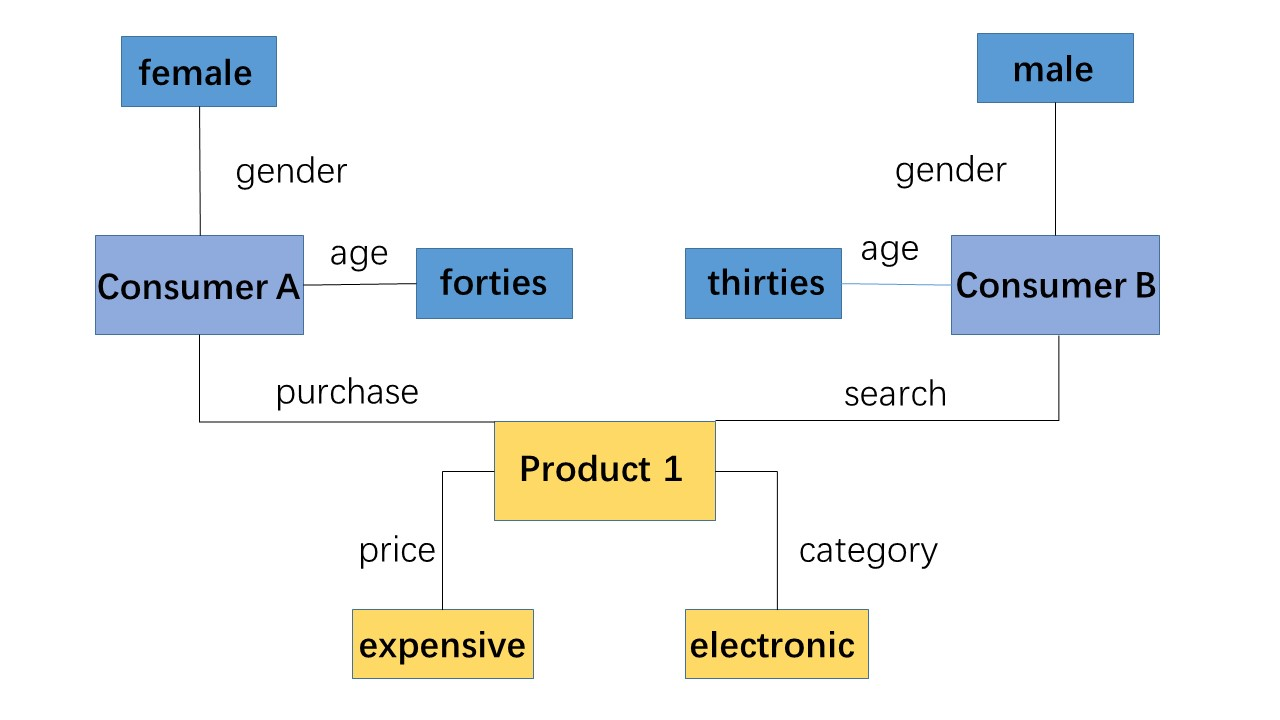
\includegraphics[width=0.50\textwidth]{er.jpg}\\
  \caption{Association Graph}\label{f1}
\end{figure}
\\
 The authors look at the expected behavior of random walk on the association graph. Based on the hitting time and commute time, the authors employ a novel measure of similarity --- the cosine correlation between states. Compared with other methods of collaborative filtering, one of the biggest advantages of random walks view is that it can incorporate large amounts of contextual information. By using cross-validation, the author proved that the random walk view collaborative filtering is more predictive and robust to perturbations of edges on the association graph than other methods. The flaw of random walk view is the heavy computing price. In that case, the authors employ approximation strategies to alleviate time complexity.
\par
Fouss et al.\cite{fouss2005a} also use random walk for movie collaborative recommendation. The authors also consider relational database as a collection of element sets linked by their connection. The authors exploit the graph structure of the relational database to compute dissimilarity measure between elements in sets. The dissimilarity is based on the hitting time and commute time. It was also the first time that hitting time and commute time measures were used in collaborative recommendation. For better understanding, the author gives us a specific example of the collaborative movie recommendation. If we get three elements, people, movie and movie category, relationships that between people and movie, and between movie and movie category. we have to do following things for movie recommendation:
\begin{itemize}
\item Compute dissimilarity measure between people based on the movies that they have watched.\\
\item Compute dissimilarity measure between people and movies for recommendation.\\
\item Compute dissimilarity measure between people and categories to give a prefer category for each person.\\
\end{itemize}
\par
As a conclusion, Fouss et al.\cite{fouss2005a} introduce a general procedure for computing similarity between elements of a relational database. These elements are not necessarily directly connected. The authors use movie recommendation as an example to show us that their method has better performance than shortest path method on recommendation. However, there are two shortcomings of the authors' method. For large databases, this method is time consuming and does not scale well. The other short coming is that the method is valid on a weighted, undirected graph.
\par
Although the random walk view of collaborative filtering is useful and has good performance, it also faces several challenges. One of the biggest problem is the start-up problem presented by Resnick \cite{Resnick1994GroupLens}. All collaborative filtering systems are based on an existed database. If there isn��t an existed database, the system can��t be built up.



\subsection{Link Prediction}

Link prediction is used to predict the links that may exist in the future of evolving networks. Link prediction problem is a long-standing challenge in both computer science community and information science community.
Random walk is one of the useful approaches to solve link prediction problem. Just like collaborative filtering, a random walk view of link prediction is also based on proximity measures.
\par
 Liben-Nowell et al. \cite{Liben2007The} present the performance of different proximity measures on link prediction problem such as hitting time and commute time, Katz score\cite{Katz1953A}, SimRank etc. They test the different measures on the coauthership network of physics. They consider that the coauthor network is evolutionary with time going by. The coauthor network is denoted by $G=<V,E>$ in which each edge $e=<u,v>$ represents coauthorship between node $u$ and node $v$ that appear at time $t(e)$. They choose four time $t_{0}, t'_{0}, t1, t'_{1}$ first. The four time has following relation: $t_{0}<t'_{0}<t_{1}<t'_{1}$. They apply algorithms in the network of $G[t_{0}, t'_{0}]$ and output a list of edges that may appear on the network in the near future. And $G[ t_{1},t'_{1}]$ are considered as the coauthorship network in the near future. They call $[t_{0}, t'_{0}]$ as the training interval and $[t_{1},t'_{1}]$ as the test interval. In order to evaluate different algorithms, they use two parameters \emph{ktraining} and \emph{ktesting} to see how accurate the new edges between two vertices can be predicted. According their results, there is no winner among the different measures. But compared with the random predictor, many methods have much better performance, which indicates that the random walk view of link prediction works. They also find that the hitting time and commute time measures suffered from the information far away. The most effective proximity measure is the \emph{Katz Score} which ensembles the paths between two nodes. Moreover, the computation of hitting time and commute time is time consuming.
 \par
 To address this problem, Sarkar et al.\cite{Sarkar2012A} come up with the idea that to replace commute time with Truncated-commute-time in link prediction task. Based on the idea, they present a novel algorithm called GRANCH\cite{Sarkar2012A} to find out which two nodes will have an edge in the near future. The main intuition of GRANCH is that consider the graph as $n$ overlapping subgraphs. Every subgraph is a bounded neighborhood for each node. And the hitting time is redefied as the random walk from any node in this neighborhood to the destination. They apply GRANCH in both simulated data and real world graphs. The authors empirically show that GRANCH reduces the computation and storage while retaining the performance of link prediction methods that based on commute time proximity measure. Link prediction also help researchers find out the potential relation between miRNAs and diseases \cite{Liu2017Inferring}. They consider the miRNA-Disease heterogeneous network as two overlapping sub-networks: miRNA similarity sub-network and diseases similarity sub-network. They employ random walk with restart to predict the miRNA-disease associations in the heterogeneous network. This is a case that random work help the biologists to do their research more conveniently.


\subsection{Recommender System }
Recommender system with random walk approaches sometimes is just like the intuition of collaborative filtering. The inherent quality is just the same. They all exploit random walk to calculate the \textbf{closeness} between vertices. One of the persuasive evidences is that there is a literature\cite{Gori2007ItemRank} comparing an algorithm for recommender system with one of the collaborative filtering algorithms presented in \cite{fouss2005a}. Hence we will give a specific application scenario to introduce the recommender system based on random walk. The scenario is recommending paper for researchers.
\par
Some scholars use random walk to solve their own problem during doing research. They find that it is hard for them to find out useful literature recently published in their field. A researcher is supposed to be well aware of recent development of the field he is working on. So a paper recommendation system can help them find out potential helpful papers which is meaningful and time saving. Because publications increase exponentially, selecting useful papers is really a pain in the neck for the most researchers.
\par
	A very simplified algorithm to solve this problem is presented by Woodruff et al.\cite{woodruff2000enhancing}. The authors employ spreading activation and citation data to generate recommendations. The authors use documents read by the reader as input. and output the most related literature to the reader in a digital book. This method only recommends a chapter or an article in a digital book.
A more applicable method for paper recommendation can be found in \cite{mcnee2002on}. The author exploit collaborative filtering for recommendation. They use the citation web as the graph to create ratings. The author investigate six algorithms by do experiments on the subset of \emph{ResearchIndex}. These algorithms can either provide relevant recommendations or novel recommendations, but none of them can do the both. And The use of citation web can affect the recommendations greatly.
\par
	Also based on the citation graph, Gori et al.\cite{Gori2007Research} exploit the idea of page rank algorithm to solve the paper recommendation problem, and devise the \emph{PaperRank} algorithm. The authors' view is that utilizing the model expressed by the citation graph can help us find out valuable papers to suggest to a user. The authors considered that the \emph{PaperRank} algorithm must have two properties: propagation and attenuation. Propagation can help us find out a paper is a good suggestion for a researcher, if the paper is relevant to good papers in bibliography of the researcher's work.
As for attenuation, it means that the positive influence of good papers decreases if we move further and further away from good papers on the citation graph. PageRank algorithm has both properties mentioned above. The author borrows its idea to solve paper recommendation problem. The essential of \emph{PaperRank} algorithm is a random-walk-based score algorithm.
\par
	Xia et al.\cite{Xia2016Scientific} incorporates author relations and historical preferences for scientific article recommendation. The authors build a graph based on the information of co-authors' relationships, and they employ the random walk with restart to generate a recommendation list. Compared with some baseline algorithms, the algorithm presented in the literature called CARE performs better in precision, recall, and F1 score. Most studies of paper recommendation use the algorithms that pay no attention to the different situation of researchers. But CARE method takes researchers�� own features into consideration. Hence the CARE method is more accurate than the baselines.

\subsection{Computer Vision}
Many researchers solve computer vision problems by using random walk. One of the popular techniques is characterizing shape of picture by using random walk. Gorelick et al. \cite{Gorelick2006Shape} compute many useful properties of a silhouette based on the notion of random walk. For every internal pixel in the contour, they compute a criterion reflecting the mean time required for a random walker beginning at the pixel to reach the boundary. Based on the computed value, they can extract many properties of the silhouette such as part structure, rough skeleton, local orientation, convex part, and concave part.
Random walk is also utilized in image segmentation.
\par
Meila et al. \cite{Meila2001A} present an approach of image clustering and segmentation based on the view of random walk proximity measures. They also find that the spectral view of clustering and segmentation have a probabilistic foundation. They exploit the eigenvalue and eigenvector of walker��s transition matrix to cluster and segment image.
\par
 Grady et al.\cite{Grady2006Random} propose a new algorithm for performing multi-label and interactive image segmentation. The interactive image segmentation means that the user has to label some pixels in the image manually. The algorithm can determine the probability of the random walker which starting from an unlabeled pixel reaching the predefined pixels. Therefore, a good segmentation of that image arises from the labels of all the pixels. The predefined labels indicate that the regions of the image belong to several objects. The authors treat the picture as a graph including nodes and edges. Nodes represents the pixels of the image. Edges represents the connection of two nodes, and the weigh of the edge means the likelihood of a random walker going through that edge. The authors believe that this view of image segmentation has two advantages: no discretization errors and no ambiguity. One reason of no discrestization is that the authors use purely combinational operators that require no discretization. The segmentation algorithm only requires the solution to a sparse, symmetric, positive definite system of equation, hence the efficiency of this algorithm is guaranteed.
 \par
 Qiu et al.\cite{qiu2005image} exploit the properties of the commute time to develop image segmentation method. They compute the commute time from the spectrum. By using the discrete Green��s function of graphs, they can analyze the cuts of the image from commute time. Qiu et al. also use commute time to motion track \cite{Qiu2006Robust}. The main purpose of using commute time as proximity measure is to alleviate the effect of noise on the shape interaction matrix. The noise on the shape interaction matrix results in the loss of block-diagonal structure and the difficulty of the assignment of elements to objects. Commute time is a more robust measure than raw proximity matrix when facing the noise on the shape interaction matrix. The authors compute the commute time by using the Laplacian matrix shown in equation \ref{lp}. They also show us that how the ensemble the commute time, kernel of PCA (Principle Component Analysis), the Laplacian eigenmap and the diffusion map. To demonstrate the result of the robust method, they compare it with some other motion tracking algorithms on synthetic and real world data. The function of commute time is to provide a proximity measure for the approaches provided by Qin\cite{Qiu2006Robust,qiu2005image}.


\subsection{Semi-supervised Learning}

Semi-supervised learning uses both labeled data and unlabeled data for training. The goal is to classify the unlabeled data when the labeled data is just a small fraction of the dataset.

Zhu et al. \cite{Zhu2003Semi} present a new approach of semi-supervised learning based on the random walk. They do classification task in continuous state space rather than in the discrete label set. The intuition of the approach is that the data points should be labeled as same as their neighbors. How to select the neighbors of a data point is a problem in front of us. The authors' strategy is to employ a harmonic function $f: V\rightarrow R$ on graph $G$. The harmonic function has a constrain on the labeled data i:
\begin{equation}
f(i) \equiv fl(i)y(i)
\end{equation}
The harmonic function, which provides a consistent probabilistic semantics, is the basis of this semi-supervised classification approach. Since the author do classification in the continuous state space, they have to turn the continuous state space into discrete label set. Instead of employing a simple threshold in terms of the interpretation of random walk, the authors incorporate the prior knowledge by using \emph{class mass normalization}(CMN) procedure. The promising result has shown that the approach can improve the accuracy of classification by exploiting the structure of unlabeled data.
\par
Szummer et al. \cite{Szummer2001Partially} the partially labeled data may be in the sub-manifold space, hence a measure of global similarity is needed for semi-supervised learning. Meanwhile, the authors also hope the measure can incorporate the structure of manifold. Based on these consideration, they present a Markov random walk model to classify the data. The research of \cite{Tishby2000Data}, which shows how to change the distance matrix into a Markov process, helps a lot with the construction of graph. In that case, the representation of data set arises naturally. Given a partially labeled data set $\{ (\mathit{X}_{1},\tilde{\mathit{y}}_{1}),\cdots,(\mathit{X}_{L},\tilde{\mathit{y}}_{L}),
\mathit{X}_{L+1},\mathit{X}_{N}\} $ in which $\mathit{L}$ is much smaller than $\mathit{N}$, the authors represent the data set as a graph where node $\mathit{k}$ represents the data $(\mathit{X}_{k},\mathit{\tilde{y}}_{k})$ or $\mathit{X}_{k}$. For node $k$, $P_{0\vert t}(i\vert k)$ denotes the probability of the random walker from node $i$ to node $k$ after $t$ steps. They classify node $k$ with the label $c$ when $c$ maximizes the following formula.
\begin{equation}
P_{post}(y\vert k) = \sum_{i}P(y\vert i)P_{0\vert t}(i\vert k)
\end{equation}
$P(y|i)$ is an unknown parameter, which can be estimated by two techniques: maximum likelihood with Expectation Maximization(\emph{EM}), and maximum margin subject to constraints. They discuss the two techniques in the paper and empirically show that the margin estimation has better performance. In a word, the authors provide a novel approach for semi-supervised learning task when the data sets with significant manifold structure. The parameter $t$ in this approach is also important. $T$, denoting the number of transitions, determines the smoothness of random walk. However, the choice of $t$ can be tricky and subjective. To overcome this little problem, Azran \cite{azran2007the} presents the rendezvous algorithm. Just the same as the work of Szummer \cite{Szummer2001Partially}, the author represents the data points as nodes of a graph and employ the random walk view to do classification. The intuition of the authors' approach is the labels�� propagation over the graph. But the rendezvous algorithm is different. The labeled points don��t propagate, but absorb the states of the random walk. The probability of each unlabeled data to be absorbed by different labeled points can be used to derive a distribution as the transition steps increase to infinity. Hence the rendezvous algorithm doesn't bother to choose a good value of the parameter $t$. The author draws a conclusion that the location of labeled point in the data set is as important as the size of labeled data set in terms of the experiments�� results.




%\subsection{Properties of Quantum walk}


\subsection{Algorithms Based on Quantum Walk}
In this section, we are going to introduce some algorithms based on the two quantum walk model mentioned above on solving practical problems. We can find some different properties between quantum walk and classical random walk through these examples. To help understand quantum walk algorithms better, we would like to separate the algorithms into two categories depending on the model they use. The first category is the continuous time quantum walk algorithm---quantum decision tree algorithm. The other category is based on discrete time quantum walk algorithms, including quantum page rank algorithm and element distinctness algorithm.


\subsubsection{Quantum Decision Tree Algorithm}\quad
\par
Fahri\cite{Farhi1997Quantum} originally presented the idea of continuous time quantum walk with the example of decision tree algorithm. He chooses the approach that systematically exploring the whole tree with a probabilistic rule. The author aims to achieve that the n-level nodes can be reach in polynomial time with a considerable probability. A tree is a penetrable tree when its node or nodes in n-level meet the requirement above. If a tree is penetrable for an specific algorithm, we believe that the problem corresponding to the decision tree is solvable with this algorithm in the polynomial time.
The author presents the quantum walk algorithm for decision tree with following intuition.
He considers decision tree nodes as quantum states in \emph{Hilbert} space. Then he constructs a Hamiltonian $\hat{H}$ which determines the time evolution of the quantum system. With the basis of Hamiltonian, the author presents the unitary time evolution operator shown in the Equation \ref{unitaryo}. The author compare quantum walk decision tree algorithm with classical counterpart, and find that there is a family of trees which are both classical penetrable and quantum penetrable. However, Some decision trees is quantum penetrable but not classical penetrable. With these findings, we can see that quantum tree algorithms is faster that classical counterparts in some occasions.
%\subsubsection{Traversal quantum algorithm}



\subsubsection{Quantum Page Rank Algorithm} \quad
\par
Page rank algorithm is one of the most important random walk algorithms. When quantum computation is widely considered in the era of random walk, it is natural and inevitable to apply quantum computation on page rank algorithm.
There is much literature  of quantum networks\cite{Elliott2004The,Peev2009The,Fujiwara2011Field,Stucki2011Long,Lancho2009QKD,langer2009standardization}. In order to study the behavior of pagerank algorithm in the quantum network, the authors present the quantum page rank algorithm\cite{paparo2012google}. However, the authors don't give a specific defination of quantum page rank algorithms, but give a admissible class shown as follows.
\begin{enumerate}
\item The classical PageRank must be embedded into the quantum class with its undirected graph structure preserved.

\item The sum of all quantum PageRanks must equal to 1.

\item The quantum PageRank obeys a quantized Markov Chain (MC) rules.

\item The classical algorithm to compute the quantum PageRank is also feasible.
\end{enumerate}
The author exploit the idea of discrete time quantum walk. Hence we have to define the coin space $H_{c}$ and Hilbert space $H_{p}$ which are mentioned in the section of discrete time quantum walk. The definition of coin space is similar to the one dimension quantum walk.


\begin{equation}
H_{c} = span\{\vert L\rangle ,\vert R\rangle\}
\end{equation}
However the Hilbert space ${H_{p}}$here is a little tricky. Since the page rank algorithm is on a graph, the author define the Hilbert space as the space of oriented edges.
\begin{equation}
H_{p} = span\{ \vert i \rangle_{1},\vert j\rangle_{2} \quad\vert \quad i,j \in N\}
\end{equation}
where N denotes the all the  vertices of the graph.  Since the edge is oriented, We use the subscript 1,2 to show the direction.

With these definition and the method of Szegedy��s Quantization of Markov Chains \cite{Richter2008Quantization}. We can present the unitatry step operator of quantum walk as follows.
%\begin{equation}
\begin{align}
U &=S(2\Pi - \mathit{1})\\
S &=\sum_{i,k=1}^{N} \vert j,k\rangle \langle  k,j\vert \\
\Pi &= \sum_{j=1}^{N} \vert \psi_{j} \rangle \langle \psi_{j}\vert \\
\vert\psi_{j}\rangle &= \vert j\rangle_{1} \otimes \sum_{k=1}^{N} \sqrt{G_{kj}}\vert k\rangle_{2}
\end{align}
%\end{equation}
Where $G_{ij}$ means the weight of edge $ij$.\\
\par
The authors apply quantum pagerank algorithm on small generated network to have a insight of the behavior of it. They find that the quantum pagerank algorithm obtain a larger score than the classical value.  In the meanwhile, the quantum algorithm break down the hierarchy of classical values. The authors also look into the properties of quantum page rank algorithm in complex real-world networks\cite{paparo2013quantum}. The authors find that quantum page rank algorithm can reveal the underlying topology of the network more univocally with respect to classical page rank algorithm.  The ability of detecting hub for network is enhanced with respect to classical counterpart.
\subsubsection{Element Distinctness}\quad
\par
We introduce the element distinctness problem first. Element distinctness problem is to tell whether all the elements in a given sequence are distinct. More precisely, $M={x_{i},i\in N}$, are there $x_{i} \in M and x_{j} in M$ and $i \neq j$ such that $x_{i}=x_{j}$? There is a simple classical algorithm to solve this problem with $Nlog(N)+O(N)$ comparisons. Buhrman et al. present an quantum algorithm to speedup\cite{buhrman2000quantum}. Their algorithm give a upper bound of computation cost $O(N^{\frac{3}{4}}log(N))$. Ambainis\cite{Ambainis2004Quantum} improve the quantum way to solve element distinctness with $O(N^{\frac{2}{3}})$ comparisons.
The intuition of this optimal quantum algorithm is to construct a graph, and transform the element distinctness problem of finding a marked vertex in the graph. In order to search marked vertex efficiently, the author improve the Grover's quantum search algorithm\cite{brassard2000quantum,grover1996a}. The author reuses the information that queries before, and search a marked vertex with $O(N^{\frac{2}{3}})$ comparisons instead of $O(N)$ comparisons in Grover's search algorithm.
\section{Open Issues}
We are in the era of information explosion. We produce so many data every day. Hence the real-world network is so giant. When we apply random walk on the giant
complex real-word network, there are two challenges in front of us. The first one is the speed of the random walk algorithms. The second one is the main-memory
volume.
\subsection{Speed of Random Walk Algorithms}
The time complexity of graph random walk kernel is at least $O(n^{3})$ or $O(m^{2})$ for graph with $n$ nodes and $m$ edges\cite{Kang2012Fast}. In an artificially generated graph, this time complexity is acceptable. But it is a disaster on a real-world network since the number of vertexes and edges is huge. It is a challenge of random walk model. There are already researchers coping with this issue. Kang et al.\cite{Kang2012Fast} propose ARK graph kernels with time complexity $O(n^{2})$ or $O(m)$. There is a prerequisite for this graph kernel. The graph must have lower intrinsic ranks than the order of the graph. Tong et al. also realize the speed problem in random walk with restart\cite{Tong2006Fast}. The algorithm of random walk with restart is slow in query time or prohibitive on storage space. The authors also exploit two properties of real-work networks: the block-wise community-like structure and the linear correlations of the adjacency matrix. With these two properties, the author devise B\_LIN approach to make random walk with restart faster. This approach preserves 90\% quality, and saves several levels of magnitude of pre-computation and storage space. As we can see, the main idea to cope with speed of random walk algorithms is to obtain approximate computation but accurate computation. We still require more accurate approximate algorithms for random walk.
\subsection{Problem of main-memory Volume}
All the fast random walk graph kernels or algorithms are under the consumption that the whole graph can be fit in the main-memory. But with the real-world
networks or graph becoming larger and larger, this condition can't be satisfied any more. One of the solutions is to divide the graph into several clusters.
There are literatures provide some approaches for graph partition and clustering on giant network.\cite{Karypis1998A,Karypis1998Metis} One of the most popular
method is METIS\cite{Karypis1998Metis}. Since more and more researchers pay attention to the giant network problem, there are a more effective clustering
algorithm for graph clustering and a better method to apply random walk on giant network with external memory\cite{Sarkar2010Fast}. The author call the
clustering method RWDISK. RWDISK has been proved to be a better way for graph partition on several famous datasets such as DBLP, citeseer and so on. But these
method still has a unacceptable time latency with respect to enormous graph. We can see that there are two ways to solve this issue, partition and using external memory.
\subsection{Computation of Hitting and Commute Time}

As we have mentioned above,  proximity measures plays an important role in network analysis and beyond. The complexity of computing commute time is $O(n^{3})$  which is prohibitive  in large graphs. There are some approximations of  commute time to reduce the complexity\cite{Sarkar2012A, Brand2005A,Spielman}. But we should be careful about these approximate approaches. These approximations can't represent the structure of large graphs or show the connectivity of vertexes in large graphs. Luxburg et al.\cite{von_luxburg2010hitting} have shown that commute time can be approximated by simple formula with high accuracy when random geometric graphs(k-nearest neighbor graphs, $\epsilon$-graphs, and Gaussian similarity graph) are large enough. More specifically, commute time $H_{uv}$ can be represented by $1/d_{u}+1/d_{v}$ in large graphs where $d_{u}$ and $d_{v}$ denote the degree of vertex $u$ and vertex $v$ respectively. Thus, the approximations only consider the local density of two vertexes but the structure information of the whole graph. The authors give two strategies to prove the result: one based on the flow argument of electric network, and the other based on spectral argument.  These two ways both prove that approximations of commute time don't take into account any global properties of large graphs.  In that case, the effectiveness of approximated commute time is doubtful. The computation of commute time in large graph is still a challenge.


\section{Conclusion}
In this paper, we introduce the random walk from the aspect of computer science. We get to know some prerequisite knowledge of understanding proximity measures based on the random walk first. Then we discuss about some classical proximity measures in a comprehensible way. Some complex variants of proximity measures we don't pay much attention to, but they won't be obstacles for us to have a whole picture of proximity measures based on random walk in our mind. We also make analytical comparison of proximity measures. We analysis the flaw of proximity measures and their application scenarios. We talk about proximity based algorithms like link prediction algorithms, collaborative filtering algorithms, and recommender systems. There are also some machine learning problems that can be well solved from the perspective of random walk. In the field of computer vision, random walk help to solve the problem of graph segmentation. In semi-supervised learning, random walk is also a effective approach. With the development of quantum computation and quantum information, the quantum view of random walk accelerates the computation of random walk algorithms significantly. Then we have discuss about the applications of quantum walks. It is exciting to find that there are many different properties and behaviours between random walk and quantum walk. We also introduce some examples that quantum walk approach can gain a remarkable speedup. Finally, we discuss problems and open issues of random walk. We focus on the problems of random walk on giant networks.






% conference papers do not normally have an appendix



% use section* for acknowledgment
\ifCLASSOPTIONcompsoc
  % The Computer Society usually uses the plural form
  \section*{Acknowledgments}
\else
  % regular IEEE prefers the singular form
  \section*{Acknowledgment}
\fi


The authors would like to thank...





% trigger a \newpage just before the given reference
% number - used to balance the columns on the last page
% adjust value as needed - may need to be readjusted if
% the document is modified later
%\IEEEtriggeratref{8}
% The "triggered" command can be changed if desired:
%\IEEEtriggercmd{\enlargethispage{-5in}}

% references section

% can use a bibliography generated by BibTeX as a .bbl file
% BibTeX documentation can be easily obtained at:
% http://mirror.ctan.org/biblio/bibtex/contrib/doc/
% The IEEEtran BibTeX style support page is at:
% http://www.michaelshell.org/tex/ieeetran/bibtex/
%\bibliographystyle{IEEEtran}
% argument is your BibTeX string definitions and bibliography database(s)
%\bibliography{IEEEabrv,../bib/paper}
%
% <OR> manually copy in the resultant .bbl file
% set second argument of \begin to the number of references
% (used to reserve space for the reference number labels box)
%\begin{thebibliography}{}
\iffalse
\bibitem{IEEEhowto:kopka}
H.~Kopka and P.~W. Daly, \emph{A Guide to \LaTeX}, 3rd~ed.\hskip 1em plus
  0.5em minus 0.4em\relax Harlow, England: Addison-Wesley, 1999.
\fi
%\end{thebibliography}
\bibliography{refer}
\bibliographystyle{IEEEtran}




% that's all folks
\end{document}


